\sectionframe{Archetypal Model}
\section{Arch}

\begin{frame}{Approach}
	\vspace{-1em}
	Construct an archetypal model with similar characteristics
	\pause
	\begin{itemize}
		\item Symmetry $F(\theta + \pi) = F(\theta) + \pi \mod 2\pi$ \hfill \cite{akyuz2022} \pause
		\item Branches $f_{\A}$ and $f_{\C}$ move up \pause
		\item The values at the left border of branches $f_{\B}$ and $f_{\D}$ move down \pause
		\item Model branches $f_\A$ and $f_\C$ quadratic \pause
		\item Model branches $f_\C$ and $f_\D$ simplified as linear
	\end{itemize}

	\begin{figure}
		\stackunder[5pt]{
			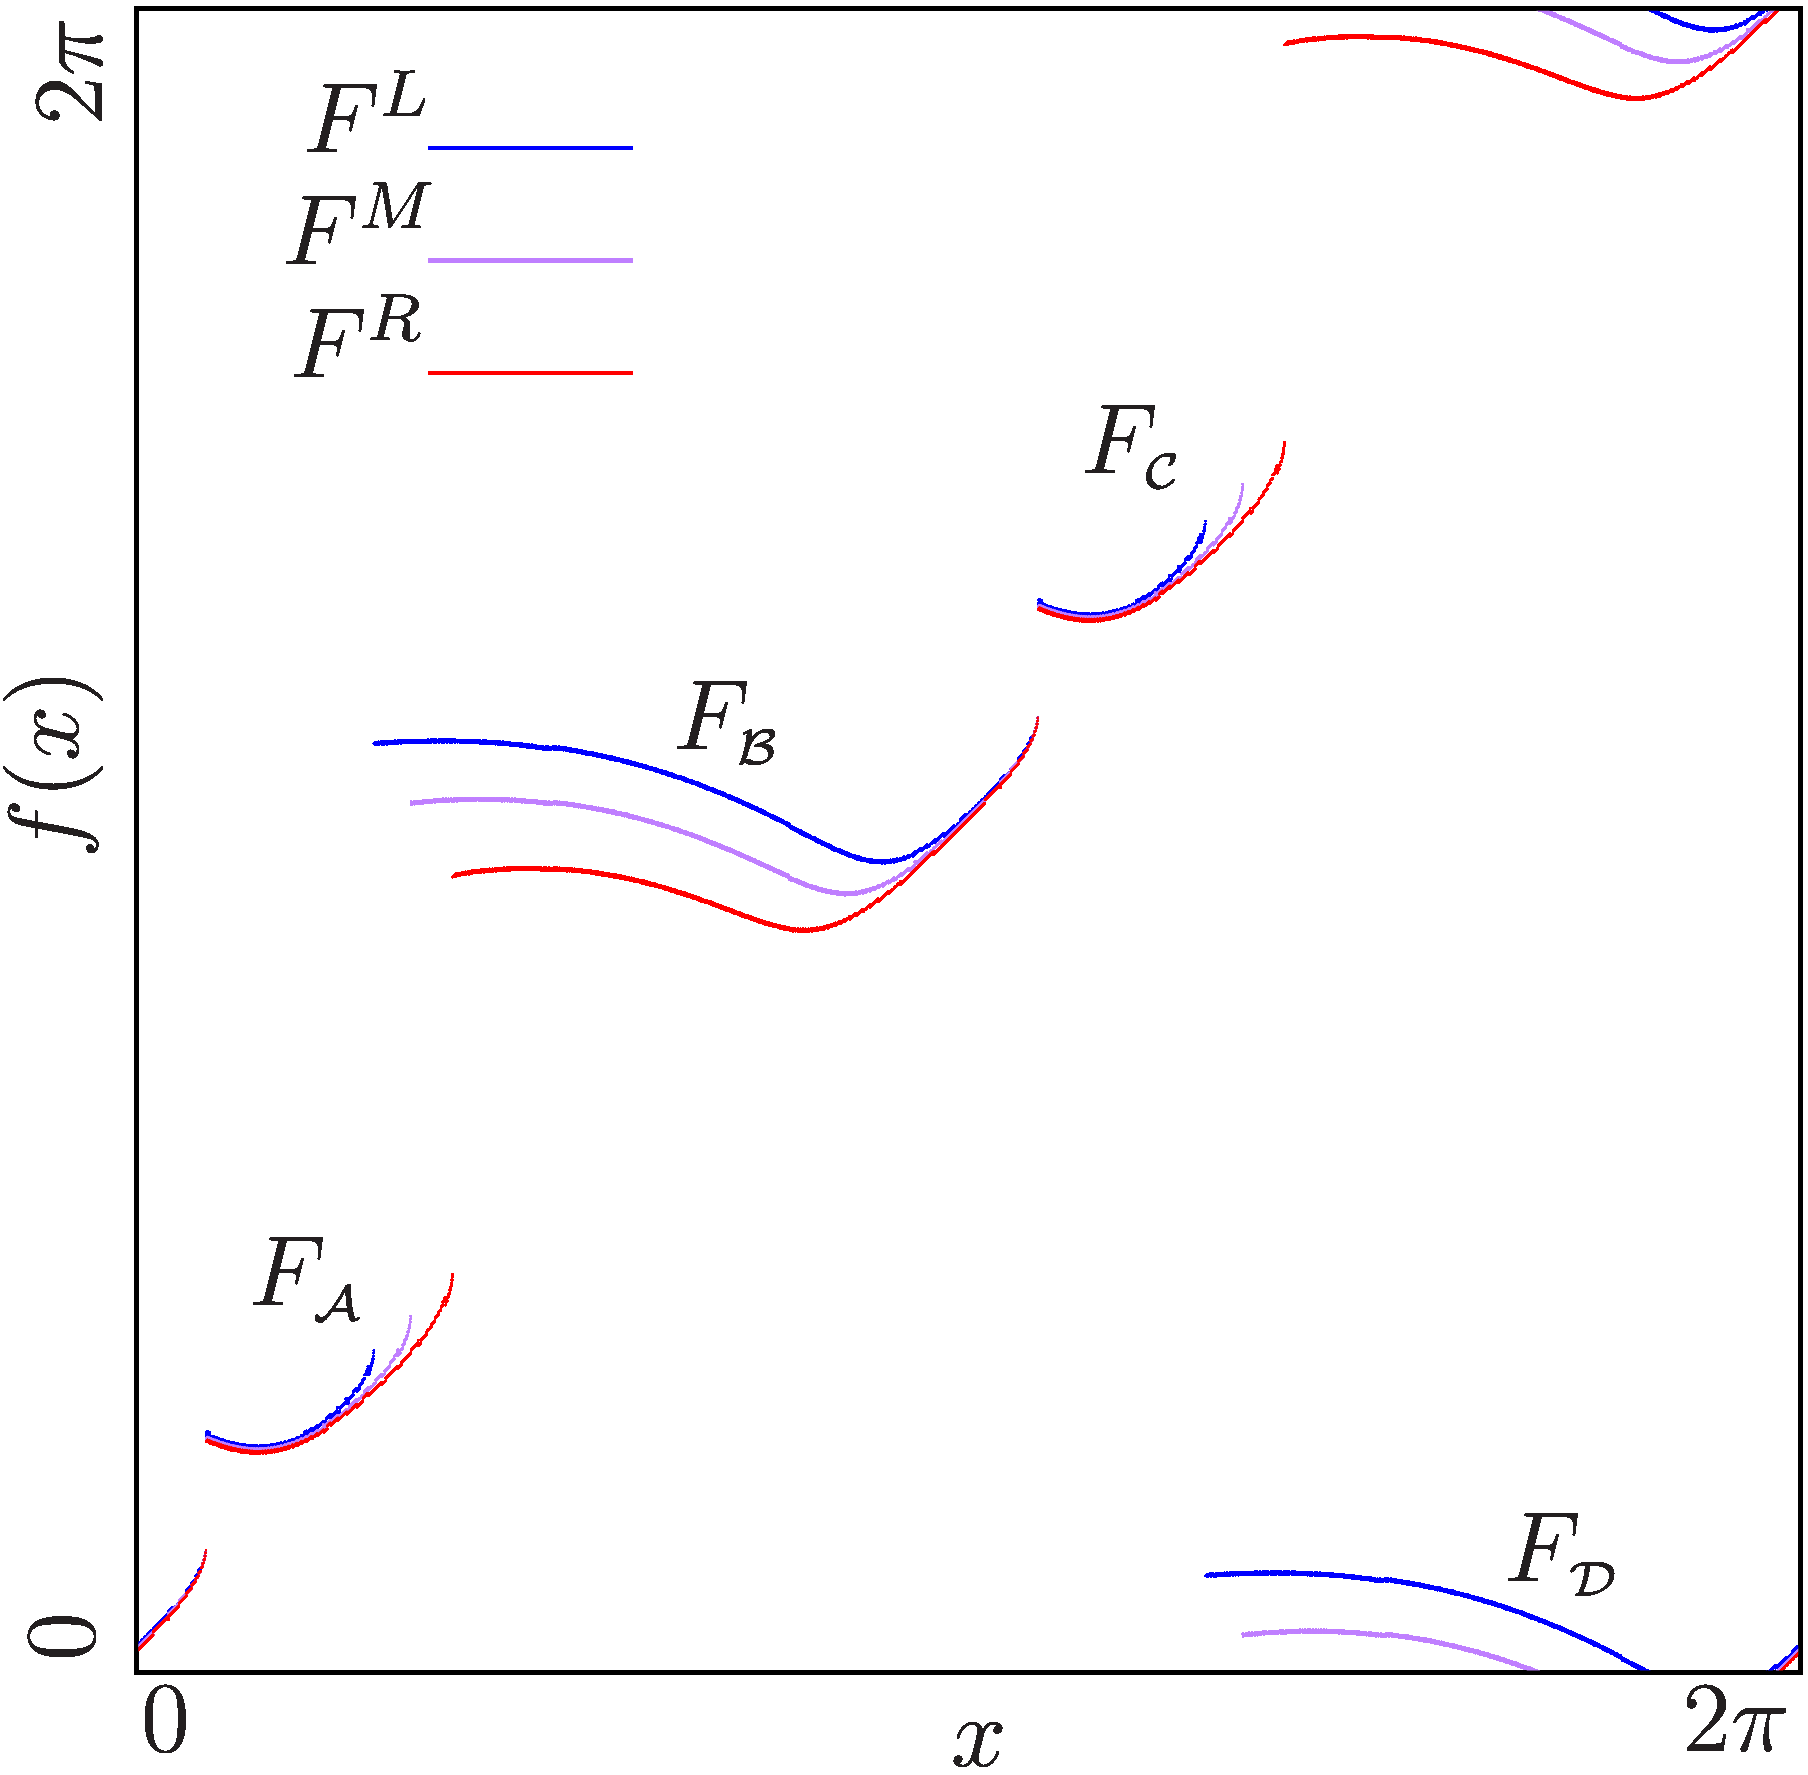
\includegraphics[width=0.2 \textwidth]{../Figures/5/5.4a/illustration.png}
		}{Effect of $E_0$}
		\stackunder[5pt]{
			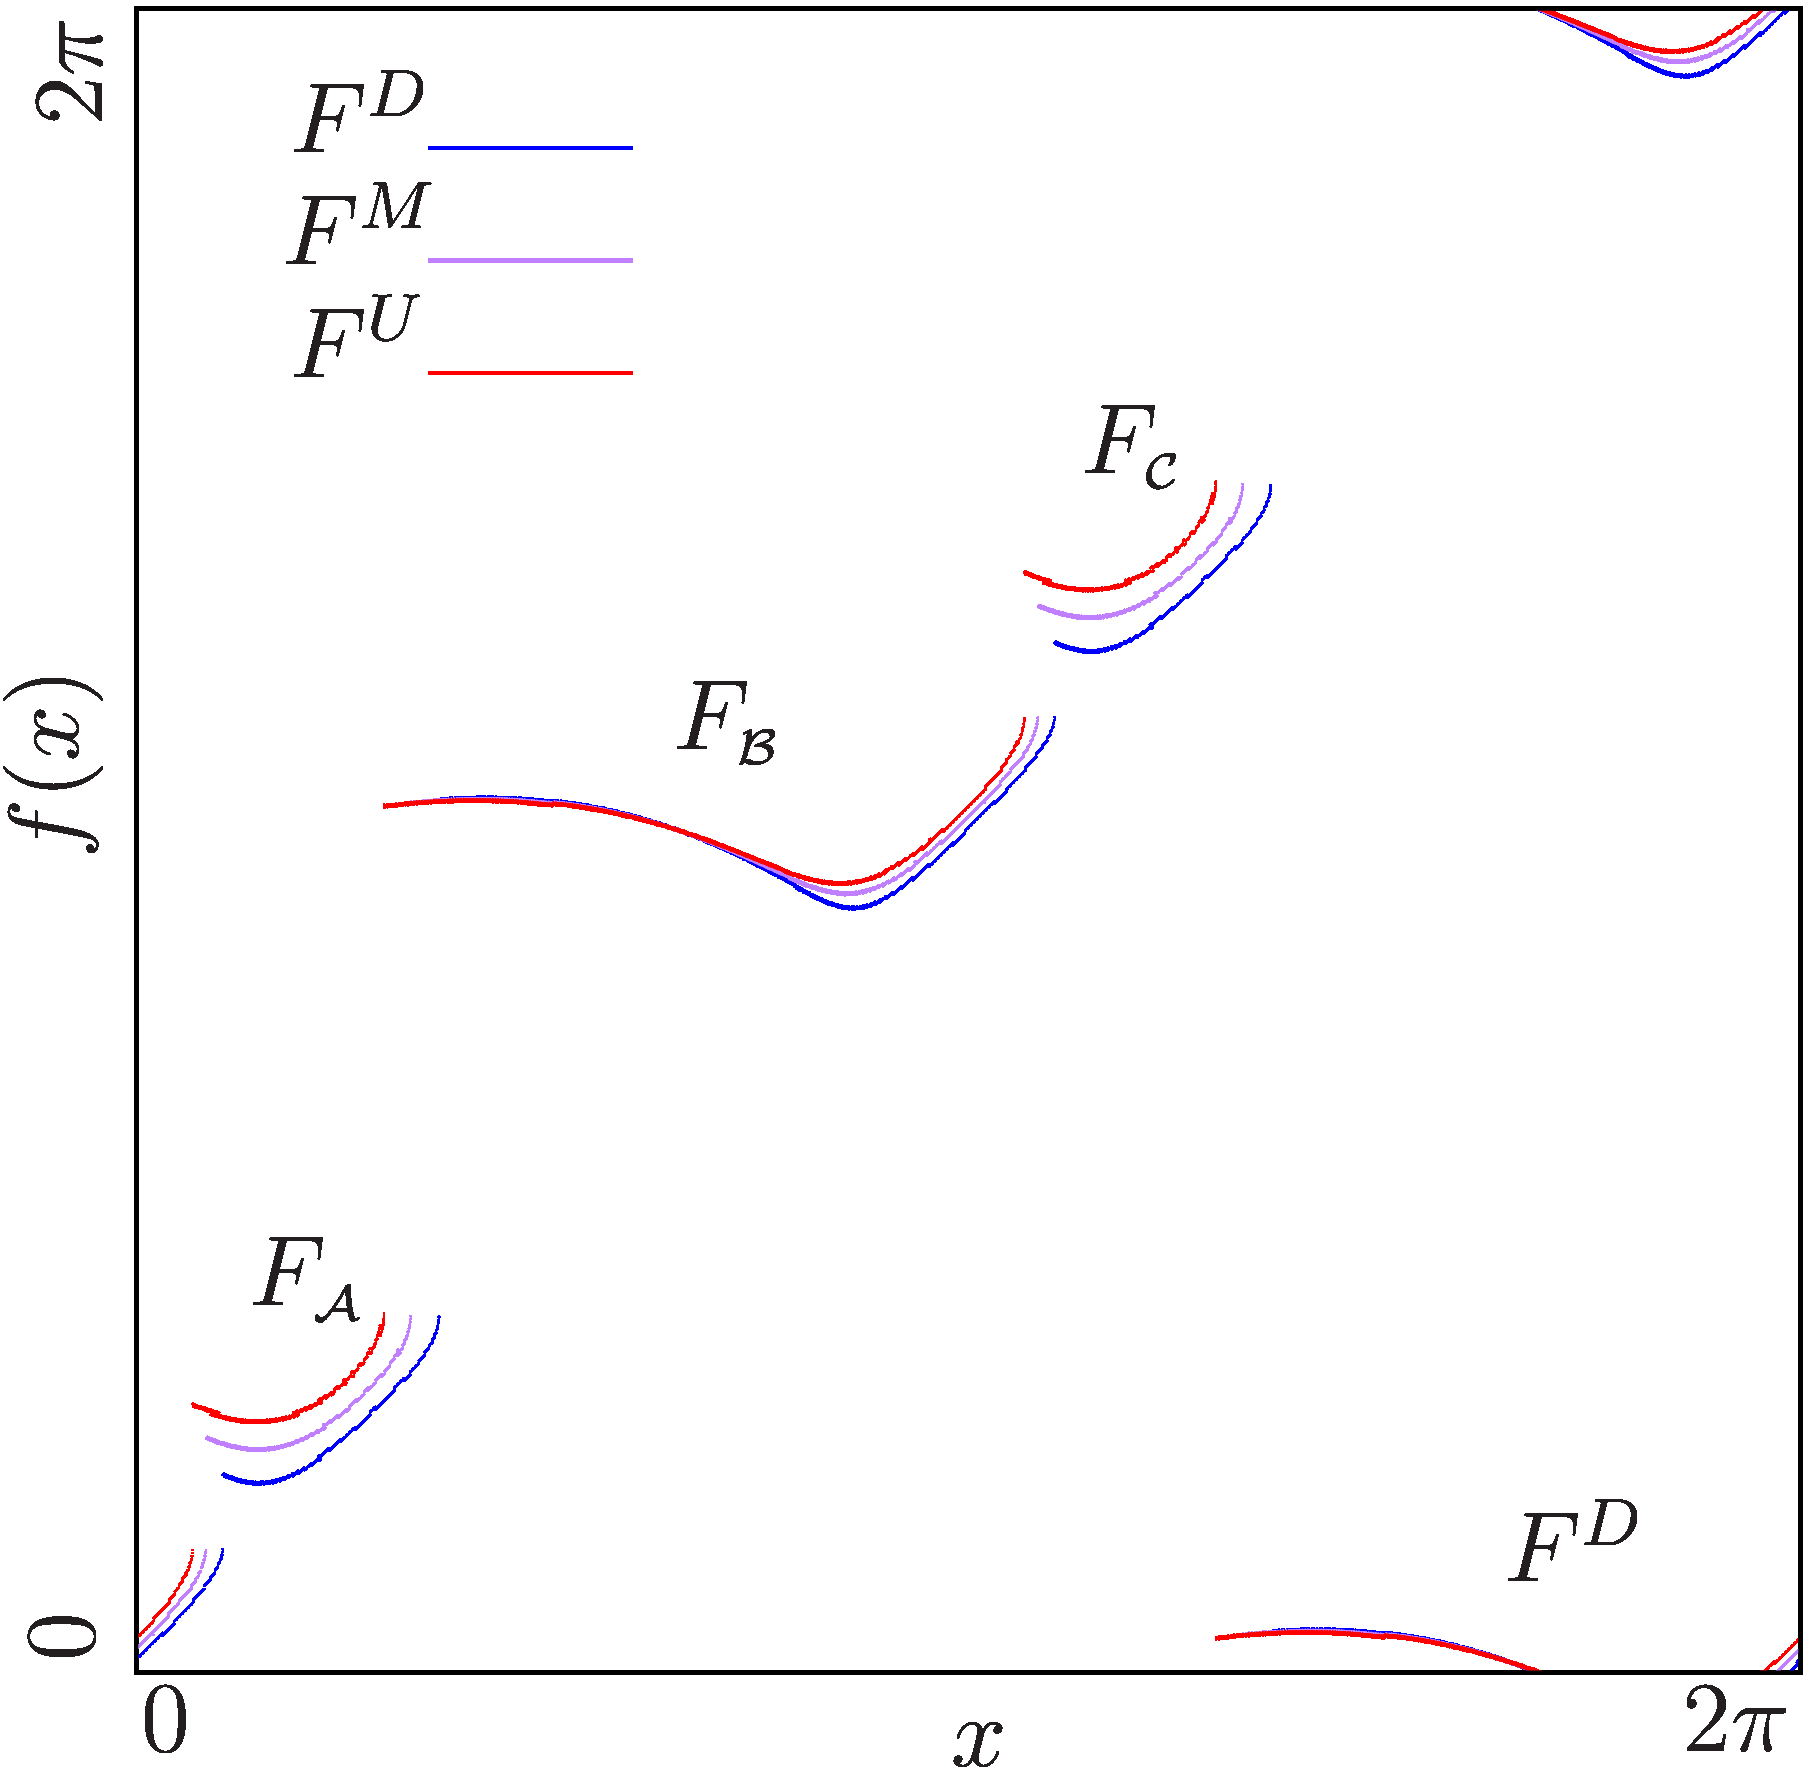
\includegraphics[width=0.2 \textwidth]{../Figures/5/5.4b/illustration.png}
		}{Effect of $\chi_0$}
		\stackunder[5pt]{
			\includegraphics[width=0.2 \textwidth]{60_MinimalRepr/ParameterEffects/p_x/illustration.png}
		}{Effect of $\alpha$}
		\stackunder[5pt]{
			\includegraphics[width=0.2 \textwidth]{60_MinimalRepr/ParameterEffects/p_y/illustration.png}
		}{Effect of $\beta$}
	\end{figure}
\end{frame}

\begin{frame}{Archetypal Model Dynamics}
	\vspace{-1em}
	\begin{figure}
		\stackunder[5pt]{
			\includegraphics[width=0.3 \textwidth]{99_Yunus/2D_Period_Zoomed/result.png}
		}{Original model}
		\qquad
		\stackunder[5pt]{
			\includegraphics[width=0.3 \textwidth]{60_MinimalRepr/2D_Period_Whole_noPoints/result.png}
		}{Simplified model}
	\end{figure}
	%With this simplified model, we explained the structures
\end{frame}

\begin{frame}{Definition of the Archetypal Model (1/2)}
	\vspace{-3.0em}
	\begin{align}
		x_{n+1} = f(x_n) \mod 1
	\end{align}

	\begin{align}
		f(x) & = \begin{cases}
			         g(x)                                        & \text{ if } x < \frac{1}{2} \\
			         g\left(x - \frac{1}{2}\right) + \frac{1}{2} & \text{ else}
		         \end{cases}
	\end{align}

	\begin{align}
		g(x) & = \begin{cases}
			         g_L(x) = a_L \cdot x^2 + b_L \cdot x + c_L & \text{ if } x < \frac{1}{4} \\
			         g_R(x) = b_R \cdot x + c_R                 & \text{ else}
		         \end{cases}
	\end{align}
\end{frame}

\begin{frame}{Definition of the Archetypal Model (2/2)}
	\vspace{-1.5em}
	\begin{columns}
		\begin{column}{.7 \textwidth}
			Fixed parameters:
			\begin{align*}
				a_L = 4 \text{ and } b_L = -\frac{1}{2}
			\end{align*}
			Variable parameters
			\begin{align*}
				 & c_L, b_R, c_R                                                                                                           \\
				\text{where} \qquad
				 & c_L = \beta,                                                                                                            \\
				 & b_R = -4 \cdot g_R\left(\frac{1}{4}\right) + 4 \cdot g_R\left(\frac{1}{2}\right),                                       \\
				 & c_R = 2 \cdot g_R\left(\frac{1}{4}\right) - 1 \cdot g_R\left(\frac{1}{2}\right),                                        \\
				\text{and} \qquad
				 & g_R\left(\frac{1}{4}\right) = \alpha, \text{and } g_R\left(\frac{1}{2}\right) = \frac{1}{2} + \epsilon \text{ is fixed}
			\end{align*}
		\end{column}
		\begin{column}{.3 \textwidth}
			\begin{figure}
				\centering
				\includegraphics[height=.5 \textheight]{60_MinimalRepr/ParameterEffects/AB/illustration.png}
				%\caption*{Illustration of the parameters $A$ and $B$}
			\end{figure}
		\end{column}
	\end{columns}
\end{frame}

\begin{frame}{The Next Step}
	\vspace{-1em}
	Research questions:
	\begin{enumerate}
		\item Is there a simple model exhibiting the same behavior? \hfill \checkmark
		\item Was there something overlooked in the analysis of the original model? \hfill \checkmark
		      \pause
		\item What else can happen in the simplified model?
	\end{enumerate}

	\pause
	\vspace{1em}
	Hypothesis: Period Adding
	\begin{itemize}
		\item This is typical for models of power converters
		\item This is typical for piecewise increasing discontinuous models
		\item This is typical in between such chains of the same period
	\end{itemize}
\end{frame}

\begin{frame}{Symbolic Sequences}
	Cycles are described using symbolic sequences.
	Symbols indicate which branches the points of the cycle are on.
	\vspace{.5em}
	\begin{columns}
		\hspace{5em}
		\begin{column}{.3 \textwidth}
			\begin{figure}
				\includegraphics[width=\textwidth]{60_MinimalRepr/Cobweb_E16/result.png}
			\end{figure}
		\end{column}
		\hspace{3em}
		\begin{column}{.6 \textwidth}
			\begin{itemize}
				\item Cycle of period 16
				\item Symbolic Sequence: $\A^5\B^3\C^5\D^3$
			\end{itemize}
		\end{column}
	\end{columns}
\end{frame}
